\documentclass[cn,10pt,math=newtx,chinesefont=founder]{elegantbook}

\title{物理學科能力競賽}
\subtitle{2021年}

\author{李宥頡}
\institute{National Taiwan University}
\setcounter{tocdepth}{3}

%\logo{logo-blue.png}
\cover{cover.jpg}

% 本文档命令
\usepackage{array}
\newcommand{\ccr}[1]{\makecell{{\color{#1}\rule{1cm}{1cm}}}}

\definecolor{customcolor}{RGB}{32,178,170}
\colorlet{coverlinecolor}{customcolor}

\begin{document}

\maketitle

\mainmatter

\chapter{物理學科能力競賽}
\section{}
%106學年度普通型高級中等學校數理及資訊學科能力競賽臺灣省中區第五區(彰雲嘉)複賽物理科理論試題

%第一題
\begin{example} 
    一長度為L的均勻繩子置於水平的桌面上,今將此繩拉直並慢慢拉出桌子邊緣,使得有一部分的繩子懸吊在桌子邊緣(如下圖一所示)。若繩與桌面之摩擦係數為$\mu$,
    \begin{enumerate}[label=(\arabic*)]
    \item 請問此系統達靜態平衡時,懸吊在桌邊之部分繩子,其最大長度為多少?
    \item 承(1),將懸吊在桌邊繩子的末端施一向下的極微小拉力,使得整條繩子向下滑,請問當整條繩子離開桌面時,其速度是多少?
    \end{enumerate}
    
    \rightline{[1]}
\end{example}

\begin{solution}
\begin{enumerate}[label=(\arabic*)]
\item $x_{max}=\mu L/(\mu+1)$
\item $v=\sqrt{\frac{gL}{\mu+1}}$
\end{enumerate}
\end{solution}

\begin{figure}[htbp]
\flushright
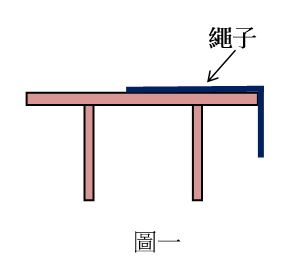
\includegraphics[width=0.4\textwidth]{image/1.JPG}
\end{figure}

\newpage


%第二題
\begin{example} 
    一質量為4m之大木塊置於一無摩擦力的水平桌面上,另一質量為m之小木塊用一不可伸縮的細繩懸吊且緊靠在大木塊的側面上(如下圖二所示),其細繩與鉛錘線之夾角為$30^o$。起初先用手托住小木塊以免其推動大木塊,然後將手放開,使二木塊開始運動。求手放開之時刻,大小二木塊的加速度$a_l$及$a_s$分別為何?(用重力加速度g表示答案) 
    
    \rightline{[2]}
\end{example}

\begin{solution}
$a_l=\sqrt{3}g/16$,$a_s=g/8$
\end{solution}

\begin{figure}[htbp]
\flushright
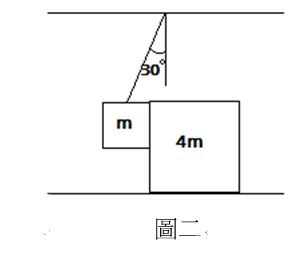
\includegraphics[width=0.4\textwidth]{image/2.JPG}
\end{figure}

\newpage


%第三題
\begin{example} 
    設地球為均勻球體(質量M、半徑R),某質點(質量$m<<M$)自地球表面以初速$v_0$、與上空鉛垂線夾角$\alpha$射出(如下圖三所示)。(假設地球靜止,不計其他外力、本題只須考慮重力。g為地表重力加速度,可令$g=\frac{GM}{R^2}$)
    \begin{enumerate}[label=(\arabic*)]
    \item 若$v_0=\sqrt{gR}$、$\alpha=0^o$質點離地表之最高距離$h=$?  
    \item 若$v_0=\sqrt{1.2gR}$、$\alpha=90^o$質點離地表之最高距離$h=$?
    \item 若$v_0=\sqrt{gR}$、$0<\alpha<90^o$質點離地表之最高距離$h=$?
    \end{enumerate}
    
    \rightline{[3]}
\end{example}

\begin{solution}

\end{solution}

\begin{figure}[htbp]
\flushright
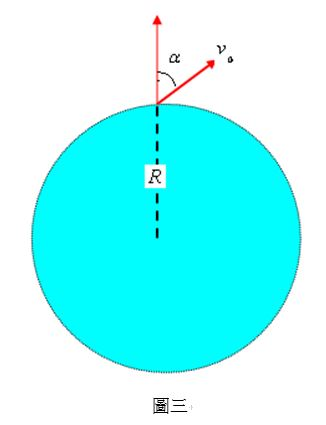
\includegraphics[width=0.4\textwidth]{image/3.JPG}
\end{figure}

\newpage


%第四題
\begin{example} 
    \begin{enumerate}[label=(\arabic*)]
    \item 如下圖四所示,一條水平弦線的一端與振動中的簧片連接,另一端繞過定滑輪,懸吊著密度為$d_1$質量為m的實心銅球,此時弦線以其第二諧頻振動。將銅球下方盛裝液體為$d_2$的容器舉高,使銅球完全浸在液體中,在此組態下,若弦線以其第三諧頻振動,求銅球半徑為何? 
    \item 今將此銅球從以上裝置卸下,改以一一長度為L,不可延展的金屬絲懸吊,並將此金屬絲的頂端固定住,質量可忽略的金屬絲懸吊,並將此金屬絲的頂端固定住。當敲擊金屬絲時,發現金屬絲會發出一基頻為f的聲音。若將此銅球三分之二的體積浸入密度為$d_2$的液體中,敲擊金屬絲時所發出的基頻的大小會為何?
    \end{enumerate}
    
    \rightline{[4]}
\end{example}

\begin{solution}
\begin{enumerate}[label=(\arabic*)]
\item $(\frac{5m}{12\pi d_2})^{1/3}$
\item $f\sqrt{1-\frac{2d_2}{3d_2}}$
\end{enumerate}
\end{solution}

\begin{figure}[htbp]
\flushright
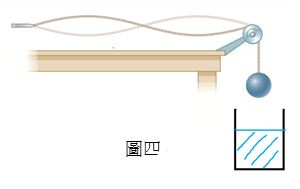
\includegraphics[width=0.5\textwidth]{image/4.JPG}
\end{figure}

\newpage


%第五題
\begin{example} 
    如下圖五所示,為由厚度$L_a$的白松木與厚度S($S=2L_a$)的磚塊所做成的隔熱牆橫切面。在白松木與磚塊之間夾著相同厚度(R)但不同熱傳導率($k_1$,$k_2$)的兩層未知材質。白松木的熱傳導率為$k_a$,而磚塊的熱傳導率為$k_s$($k_s=5k_a$)。牆的表面積為A。試問:
    \begin{enumerate}[label=(\arabic*)]
    \item 在物理學中穩態的情況下,當通過牆的熱傳導達到穩態的情況下,$T_1=25^oC$,$T_2=20^oC$及$T_5=-10^oC$時,$T_4$的溫度為何?
    \item 在物理學中穩態的情況下,如果將兩個不同熱傳導率($k_1$,$k_2$)的夾層,放置位置互換,$T_3$的溫度會不會改變?導出$T_3$的大小與$k_1$,$k_2$,$T_2$及$T_4$的關係(在物理學中穩態中$T_2$及$T_4$為已知)。\item 現在設計一個保溫屋,在寒冷天氣下,讓室內保持室溫。從(1)(2)題目敘述及熱傳導的角度,在下圖的結構中,如果兩個不同熱傳導率夾層的厚度保持不變 (R固定),何種條件設計可以達成此目的?並說明你設計的物理解釋(限50字內)
    \end{enumerate}
    
    註:熱傳導速率$P_{con}=\frac{Q}{t}=kA\frac{T_H-T_L}{L}$,Q:所轉移的熱量
    
    \rightline{[5]}
\end{example}

\begin{solution}
\begin{enumerate}[label=(\arabic*)]
\item $-8^oC$
\item $T_3=\frac{k_1T_2+k_2T_3}{k_1+k_2}$
\item 可以利用較小的$k_1$及$k_2$隔熱材質來完成。由於從屋內到屋外熱量的傳遞,經過熱傳導率低的介質的熱量傳遞的速率較慢。兩個介質交換位置並不會影響,主要是介質厚度。
\end{enumerate}
\end{solution}

\begin{figure}[htbp]
\flushright
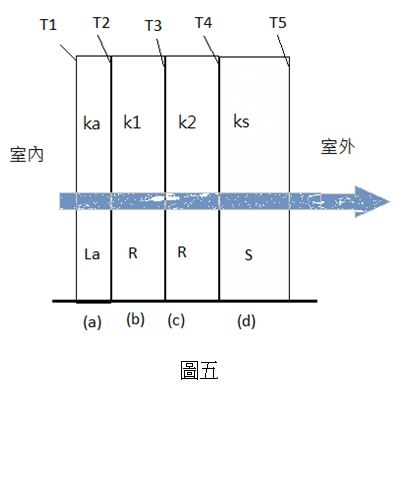
\includegraphics[width=0.5\textwidth]{image/5.JPG}
\end{figure}

\newpage


%第六題
\begin{example} 
    \begin{enumerate}[label=(\arabic*)]
    \item 二個相同之薄平凸透鏡互相對組,凸面朝內且鏡心互相接觸,空隙部分灌入折射率1.65之液體。平凸透鏡之折射率為1.55,曲率半徑為20公分。求當一物體置於此組合元件之左方無限遠處,則成像位置為何?
    \item 一個發散薄透鏡及一平凹面鏡具有相同之焦距10公分,一物體置於發散薄透鏡左方15公分處,且平凹面鏡置於發散薄透鏡右方30公分處。求此物體之成像相對於發散薄透鏡之位置?
    \end{enumerate}
    
    \rightline{[6]}
\end{example}

\begin{solution}
\begin{enumerate}[label=(\arabic*)]
\item 於此組合元件之左方100公分處。
\item 透鏡右方6.18公分。
\end{enumerate}
\end{solution}

\newpage


%第七題
\begin{example} 
    考慮一個He-Ne氣體雷射光學共振腔,其光學共振腔長度為40cm,雷射光於共振腔中形成駐波,然後由一端出口離開共振腔。由於Ne氣體原子在受激發的情況下會一邊運動一邊發射出中心波長($\lambda_0$)為632.8nm的雷射光,因此在計算共振腔所發出的雷射光波長時,就必須同時考慮Ne原子運動所造成之督卜勒效應,與光學共振腔所能提供的駐波膜態的影響。假設Ne氣體原子以均方根速度($v_x$)為406$m/s$沿x軸行進,對於所發射之雷射光在頻譜上的貢獻為拓寬其頻譜(Doppler broadened)使其頻譜半高寬擴增為$\Delta f_{1/2}=\Delta f_{rms}$($=2f_0v_x/c$,其中$f_0$為中心頻,c為光速)。求:
    \begin{enumerate}[label=(\arabic*)]
    \item 中心頻率$f_0$為多少?
    \item 頻譜半高寬$\Delta f_{rms}$為多少?
    \item 波長半高寬$\Delta \lambda_{1/2}$為多少?(提示:$\Delta \lambda_{1/2}/\Delta f_{rms}$等於$d\lambda/df$為$\lambda$對f的微分)
    \item 不同的共振膜態間,其膜態波長差距$\Delta \lambda_m$多少?
    \item 那麼這樣一個雷射共振腔大約可以有幾種雷射膜態?其波長分別為多少?
    \end{enumerate}
    
    \rightline{[7]}
\end{example}

\begin{solution}
\begin{enumerate}[label=(\arabic*)]
\item $4.74*10^{14}/s$
\item 1.28GHz
\item 1.65pm
\item 0.501pm
\item 3種($1.65/0.501=3$),分別是632.3nm, 632.8nm, 633.3nm
\end{enumerate}
\end{solution}

\begin{figure}[htbp]
\flushright
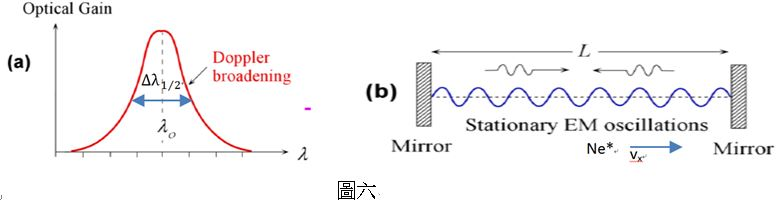
\includegraphics[width=1.0\textwidth]{image/6.JPG}
\end{figure}

\newpage





%106學年度普通型高級中等學校數理及資訊學科能力競賽第9區複賽物理科筆試參考解

%第一題
\begin{example} 
    某日太陽、月球及地球的相對位置如圖一,已知太陽的質量為$1.98*10^{30}$公斤,月球的質量為$7.34*10^{22}$公斤,太陽距離地球$R_s=1.496*10^{11}$公尺,月球距離地球為$R_m=3.84*10^8$公尺,地球半徑為$R_E=6.37*10^6$公尺。
    \begin{enumerate}[label=(\arabic*)]
    \item 計算月球對地球的引力及太陽對地球的引力比值的絕對值。
    \item 計算月球對地表A處與D處的引力差值及太陽對地表A處與D處的引力差值之比值的絕對值(提示:因$R_s>>R_E$且$R_m>>R_E$,取差值可取至$R_E/R_m$的一次項即可,並利用此數學近似:${(1+x)}^n\approx 1+nx$當$x\approx 0$)。
    \item 由(1)及(2)的計算結果來評論月球或太陽對潮汐現象的影響何者較大?
    \item 將地球描繪成如上圖之圓形,於此圓外描繪地球上的海水(潮汐)高度分佈(請記得標上點A,B,C,D於圓上)。
    \item 某觀測者於傍晚6點時位於點C的海岸邊,試問傍晚6點到7點時該觀測者所見的月亮形狀(畫圓並標明亮、暗區)及潮汐現象(漲潮或退潮)?
    \end{enumerate}
    
    \rightline{[1]}
\end{example}

\begin{solution}
\begin{enumerate}[label=(\arabic*)]
\item 0.00563 (or $1/177.73$)
\item 2.19 (or 2.21)
\item 由(2)知月球對潮汐現象的影響較大,因為潮汐現象和各處的重力差有關,和重力的絕對大小無關。
\item 
\item 
\end{enumerate}
\end{solution}

\begin{figure}[htbp]
\flushright
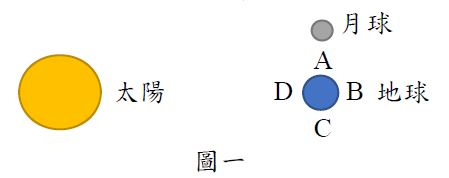
\includegraphics[width=0.5\textwidth]{image/11.JPG}
\end{figure}

\newpage


%第二題
\begin{example} 
    一均勻木棒斜放於一內含某種液體的容器(如圖二所示),$3/5$的棒長沉於一面底下,棒子另一端固定於一可自由轉動的軸上。
    \begin{enumerate}[label=(\arabic*)]
    \item 找出液體和棒子的密度比值。
    \item 用手稍微增大棒子和器壁的夾角再放開,棒子開始會於原平衡位置附近震盪,若以同設備但改變液體密度為原液體密度的兩倍,忽略液體流動及黏滯力的效應,新的震盪週期(A)較原震盪週期大(B)較原震盪週期小(C)和原震盪週期相同。選A或B或C,請簡單解釋你的理由。
    \item 用手稍微增大棒子和器壁的夾角再放開,棒子開始會於原平衡位置附近震盪,若以同設備同液體但將此實驗移至月球表面上進行,忽略液體流動及黏滯力的效應,新的震盪週期(A)較原震盪週期大(B)較原震盪週期小(C)和原震盪週期相同。選A或B或C,請簡單解釋你的理由。
    \end{enumerate}
    
    \rightline{[2]}
\end{example}

\begin{solution}
\begin{enumerate}[label=(\arabic*)]
\item $\frac{25}{21}$
\item (A);題(2)及下題(3)是簡諧振盪的應用,可以單擺(擺線長L)於重力加速度g 的重力場週期:$T=2\pi \sqrt{\frac{L}{g}}$來想,本題中等效重力場的方向是沿著棒子的(平衡位置)方向,當液體密度增加時棒子及器壁的夾角增加,故等效重力g減少,因此週期增加。
\item (A);月球的重力加速度是地球的1/6,故週期增大
\end{enumerate}
\end{solution}

\begin{figure}[htbp]
\flushright
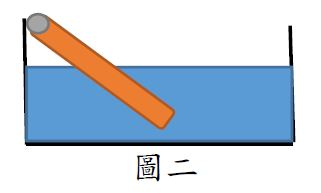
\includegraphics[width=0.3\textwidth]{image/22.JPG}
\end{figure}

\newpage


%第三題
\begin{example} 
    如圖三,在仰角$30^o$的斜面上斜向拋射一質點,質量為2kg,初速$v_o=7.5m/s$ 垂直斜面。若斜面夠長,質點落於斜面上(重力加速度$g=10m/s^2$)。
    \begin{enumerate}[label=(\arabic*)]
    \item 質點落於斜面上的位移大小為何?
    \item 質點飛行過程中任意區間,重力做功之最大量值為何?
    \item 質點飛行過程中,俯角為$37^o$時飛行軌跡之曲率半徑為何?
    \end{enumerate}
    
    \rightline{[3]}
\end{example}

\begin{solution}
\begin{enumerate}[label=(\arabic*)]
\item 7.5 m
\item 117.188 J
\item 2.747 m
\end{enumerate}
\end{solution}

\begin{figure}[htbp]
\flushright
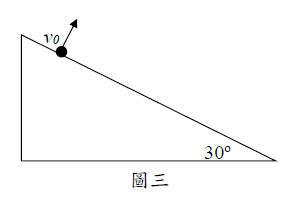
\includegraphics[width=0.4\textwidth]{image/33.JPG}
\end{figure}

\newpage


%第四題
\begin{example} 
    質量M半徑為R之實心球以初角速度$\omega$繞水平軸轉動(轉動慣量為$\frac{2}{5}MR^2$),如果它垂直掉落於地面且沒有彈跳,經t秒後做純滾動。
    \begin{enumerate}[label=(\arabic*)]
    \item 求地面與球面之間的動摩擦係數。(以重力場強度g、R、$\omega$及t表示)
    \item 球落地到做純滾動之角位移為何?(以$\omega$及t表示)
    \item 球落地經過2t秒,過程中摩擦力作功為何?(以M、R及$\omega$表示)
    \end{enumerate}
    
    \rightline{[4]}
\end{example}

\begin{solution}
\begin{enumerate}[label=(\arabic*)]
\item $\mu=\frac{2R\omega}{7gt}$
\item $\theta=\frac{9}{14}\omega t$
\item $W=-\frac{MR^2\omega^2}{7}$
\end{enumerate}
\end{solution}

\newpage





%106學年度普通型高級中等學校數理及資訊學科能力競賽臺灣省第6 區複賽物理科筆試參考解

%第一題
\begin{example} 
    如圖所示,一個3kg的木塊靜止於仰角$37^o$的斜面上,木塊與斜面之間的摩擦係數$\mu=0.4$。其中一端以質量可忽略不計的細線捲繞在質量與半徑分別為1kg與10cm的實心轉輪上,轉軸阻力可忽略。(重力加速度$g=10m/s^2$,轉輪之轉動慣量$I(=MR^2/2)$需自行計算出量值。)
    \begin{enumerate}[label=(\arabic*)]
    \item 木塊釋放後,轉輪的角加速度為多少弧度/秒$^2$?
    \item 木塊自釋放經2秒,重力做功為多少焦耳?
    \end{enumerate}
    
    \rightline{[1]}
\end{example}

\begin{solution}
\begin{enumerate}[label=(\arabic*)]
\item $24 rad/s^2$
\item 86.4 J
\end{enumerate}
\end{solution}

\begin{figure}[htbp]
\flushright
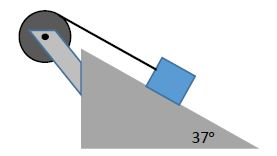
\includegraphics[width=0.4\textwidth]{image/111.JPG}
\end{figure}

\newpage


%第二題
\begin{example} 
    如圖所示,光滑平行導軌abcd與efgh,軌道的水平部分處於鉛直向上的均勻磁場中,ab段軌道寬度為cd軌道寬度的2倍($\overline{ab}=\overline{bf}=2\overline{cg}=2\overline{dh}$),軌道足夠長。將質量均為m的金屬棒P和Q分別置於軌道的ab段和cd段,將P從距離水平面軌道高度為L的地方由靜止釋放,使其自由下滑。當金屬棒P進入軌道的水平部分(磁場區域),一開始會產生感應電流在兩金屬棒與軌道形成的迴路中。
    \begin{enumerate}[label=(\arabic*)]
    \item 當金屬棒P滑至水平ab段,且到達等速。此時金屬棒P和金屬棒Q的速度大小比值為何?
    \item 承(1),金屬棒P速度大小為何?
    \item 當金屬棒P滑入cd段經2秒再次到達等速,此2秒內金屬棒Q所受之平均磁力大小為何?
    \end{enumerate}
    
    \rightline{[2]}
\end{example}

\begin{solution}
\begin{enumerate}[label=(\arabic*)]
\item $\frac{v_P}{v_Q}=\frac{1}{2}$
\item $v_P=\frac{\sqrt{2gL}}{5}$,$v_Q=\frac{2\sqrt{2gL}}{5}$
\item $\frac{m\sqrt{2gL}}{10t}$
\end{enumerate}
\end{solution}

\begin{figure}[htbp]
\flushright
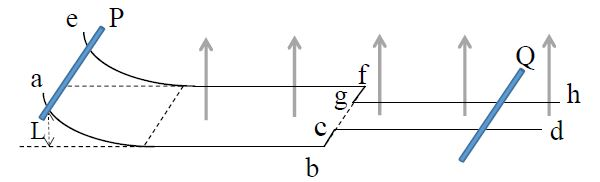
\includegraphics[width=0.9\textwidth]{image/222.JPG}
\end{figure}

\newpage


%第三題
\begin{example} 
    \begin{enumerate}[label=(\arabic*)]
    \item 下圖右側為一個半徑為R,質量為2m的四分之一圓弧狀光滑木塊(如灰色區域所示),緊靠在光滑的地面與牆上,將一質量為m的A質點從木塊頂端靜止釋放。求當木塊受牆面之最大正向力時,質點與圓心之連線與鉛直線的夾角為何?
    \item 下圖左側為一個彈簧系統,由力常數為k的一條彈簧(質量不計)和兩個質量同為m的B質點與C質點所組成,C質點輕靠牆壁。滑下木塊的A質點自右方撞向此彈簧系統,若碰撞後A質點與B質點就一直連在一起,且因牆壁之作用力,最後彈簧及三質點會一起向右運動,試求在C質點離開牆壁後的水平運動期間,彈簧長度的最大變化量為何?(以m,g,k,R表示之)
    \item 若在上述的碰撞前,B質點與C質點的質量分別改為2m與3m,A質點質量不變,當經過與上述相同的過程後,請問此次彈簧長度的最大變化量是前一小題情況的幾倍?
    \end{enumerate}
    
    \rightline{[3]}
\end{example}

\begin{solution}
\begin{enumerate}[label=(\arabic*)]
\item $45^o$
\item $x=\sqrt{\frac{mgR}{3k}}$
\item $x=\sqrt{\frac{mv^2}{6k}}$,為前一小題情況的1倍
\end{enumerate}
\end{solution}

\begin{figure}[htbp]
\flushright
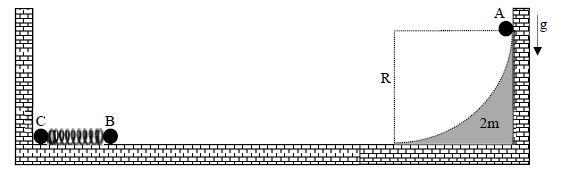
\includegraphics[width=0.9\textwidth]{image/333.JPG}
\end{figure}

\newpage


\begin{example} 
    使平行板電容器$C_1$充電至電位差為$V_0$,便將充電之電池移走,並將此電容器與一未充電的平行板電容器$C_2$相連(電容器$C_2$為將介電常數$\kappa=3$的物質填入與$C_1$相同的平行電容器極板間之左半部分),如圖所示,試問:
    \begin{enumerate}[label=(\arabic*)]
    \item 當開關S連接後,電容器$C_1$的電位差為何?
    \item $C_2$極板上的電荷量為$C_1$電荷量的幾倍?
    \item 開關S連接後,系統所儲存的能量是開關連接前的幾倍?
    \end{enumerate}
    
    \rightline{[4]}
\end{example}

\begin{solution}
\begin{enumerate}[label=(\arabic*)]
\item $V=\frac{1}{3} V_0$
\item $C_2$的電荷量為$C_1$的2倍
\item 開關S連接後,系統所儲存的能量是開關連接前的$\frac{1}{3}$
\end{enumerate}
\end{solution}

\begin{figure}[htbp]
\flushright
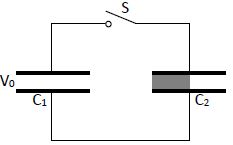
\includegraphics[width=0.4\textwidth]{image/444.JPG}
\end{figure}

\newpage





%106學年度普通型高級中等學校數理及資訊學科能力競賽高雄區複賽物理科筆試試題及參考解

%第一題
\begin{example} 
    如下圖,質量為m的質點從高度為h的光滑斜面下滑至光滑地面,與一垂直地面的均勻細棒碰撞並黏附其上,細棒一端懸掛在支點O上,另一端接近地面但並未接觸,其長度為l,質量為M,若細棒繞支點O旋轉的最大角度為60度,且$M=m$,請問h是l的幾倍?(均勻細棒繞著支點O旋轉的轉動慣量為$\frac{1}{3} Ml^2$)
    
    \rightline{[1]}
\end{example}

\begin{solution}
h是l的1倍
\end{solution}

\begin{figure}[htbp]
\flushright
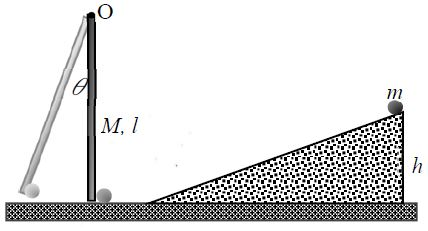
\includegraphics[width=0.5\textwidth]{image/1111.JPG}
\end{figure}

\newpage


%第二題
\begin{example} 
    如下圖所示,在光滑平面上有一質量為m的質點以初速$v_0$且方向與x軸夾角45度射向一半徑為R且質量為M的靜止光滑圓環,若質點與圓環發生完全彈性碰撞,且碰撞時間極短忽略不計,試求:
    \begin{enumerate}[label=(\arabic*)]
    \item 質點從開始出發到第三次與圓環碰撞,所經過的時間為何?
    \item 承上題,當發生第三次碰撞時,若此時圓環中心與最初始中心位置的距離為半徑的$\sqrt{5}$倍,請問M是m的幾倍?
    \item 若在一開始時將M變為原來的6倍,m變為原來的3倍,R與$v_0$皆變為原來的2倍,請問在這種情況下,第一次與第二次碰撞所間隔的時間將變為原來的幾倍?
    \end{enumerate}
    
    \rightline{[2]}
\end{example}

\begin{solution}
\begin{enumerate}[label=(\arabic*)]
\item $\frac{3\sqrt{2}R}{v_0}$
\item M是m的1倍
\item 第一次與第二次碰撞所間隔的時間與M及m無關,若R與$v_0$皆變為原來的2倍,則時間間隔將為原來的1倍。
\end{enumerate}
\end{solution}

\begin{figure}[htbp]
\flushright
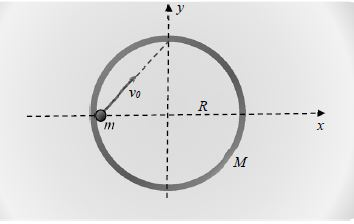
\includegraphics[width=0.5\textwidth]{image/2222.JPG}
\end{figure}

\newpage


%第三題
\begin{example} 
    甲乙兩人玩追逐遊戲,先在地上畫一半徑為R的大圓,甲以v的等速率沿著圓周跑,乙從圓心o出發以u($u<v$)的等速率追著甲跑。經過一段時間後,乙宣稱他與甲的距離變成固定值不再改變。請問乙所說的可能嗎?如果可能,請算出此距離;如果不可能,請說明理由。
    
    \rightline{[3]}
\end{example}

\begin{solution}
距離是$R\sqrt{1-(\frac{u}{v})^2}$
\end{solution}

\newpage


%第四題
\begin{example} 
    三顆金屬球甲、乙、丙,其質量分別為m、3m、m,所帶電荷均為q。三顆球以兩條長度為d之輕的絕緣線連接,並放置在水平無摩擦及絕緣的桌面上。原本三顆球都靜止並形成一直線,如下圖所示,接著一個短暫的水平推力作用於乙球,使其擁有一垂直於絕緣線方向的初速度v。請問在後來的運動中,甲丙兩球最小距離是多少?(庫倫常數為K)
    
    \rightline{[4]}
\end{example}

\begin{solution}
$D=\frac{10dKq^2}{6dmv^2+5Kq^2}=\frac{2d}{1+6dmv^2/5Kq^2}$
\end{solution}

\begin{figure}[htbp]
\flushright
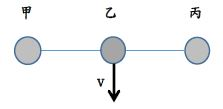
\includegraphics[width=0.4\textwidth]{image/4444.JPG}
\end{figure}

\newpage



\end{document}